% =============================================================
%  Question3.tex —— 问题三：面向 50 客户的大规模单车辆路径规划
%  数据来源：results/基础模型/q3_pure_python.json
%             results/基础模型/q3_kaiwu_sdk.json
%             results/真机结果/q3/  (seg2 / seg3)
%             paper/章节/00_实验日志_问题三.md
%  编译方式：xelatex Question3.tex
% =============================================================
\documentclass[UTF8,12pt,a4paper]{ctexart}

\usepackage{amsmath}
\usepackage{amssymb}
\usepackage{geometry}
\geometry{margin=2.5cm}
\usepackage{booktabs}
\usepackage{float}
\usepackage{caption}
\usepackage{graphicx}
\graphicspath{{../../../figures/}}

% 与全文章节编号对齐：本节在主稿中为第 8 节
\setcounter{section}{7}

\begin{document}

% =============================================================
\section{问题三：面向 50 客户的大规模单车辆路径规划}
\label{sec:q3}
% =============================================================

% -------------------------------------------------------------
\subsection{问题三分析与规模挑战}
% -------------------------------------------------------------

问题三沿用问题二的软时间窗评价函数（罚系数 $M_1=10,\ M_2=20$，无空闲等待），但客户规模
由 $n=15$ 扩展为 $n=50$。模型结构本身与问题二完全相同——单车辆 TSPTW、综合目标
$J=\mathrm{travel}+\sum_i P_i(t_i)$——但规模放大十余倍后引出两个新挑战：
（i）one-hot 全局编码所需的 QUBO 比特数变为 $n^{2}=2\,500$，远超玻色 CPQC-550 真机的
550 比特上限，全局 QUBO 既不可上传至真机，SDK 端 SA 求解的可行率亦逼近 0；
（ii）时间窗结构性紧张被进一步放大，多数客户的迟到不可避免，业务目标退化为"在不可避免
的违反中尽量减少惩罚"。本问的核心贡献因此不在于"跑出 50 客户最短路"，而在于：
在真机 550 比特限制下设计一套\textbf{可上传、可分解、可拼接、可回评}的 subQUBO 求解
流水线，并通过 Python / Kaiwu SDK / CIM 真机的多层交叉验证给出一致结果。

% -------------------------------------------------------------
\subsection{全局 QUBO 变量规模与比特预算}
\label{subsec:q3-budget}
% -------------------------------------------------------------

直接套用问题一的全局 one-hot 编码 $x_{i,p}\in\{0,1\}$（$i,p=1,\dots,n$，$n=50$）需要
$n^{2}=2\,500$ 个二进制变量，对应 Ising 维度约 $2\,501$。该规模已超过 CPQC-550 真机比特
上限近 4.5 倍，无法直接上传；同时全局 QUBO 在 SDK SA 上的合法 one-hot 排列占比
$\sim 50!/2^{2500}$，可行率极低。本文据此放弃全局 one-hot，采用"\textbf{经典启发式提供
强基线 $\to$ 滚动切片 subQUBO $\to$ 分段独立求解 $\to$ 拼接回评}"的分解框架。各编码
方案的比特预算对比汇总于表~\ref{tab:q3-budget}。

\begin{table}[H]
  \centering
  \caption{问题三 QUBO 编码方案比特预算对比（550 为 CPQC-550 真机比特上限）}
  \label{tab:q3-budget}
  \footnotesize
  \begin{tabular}{lccccl}
    \toprule
    编码方案 & 变量数 & $\le 550$ & SDK 可求性 & CIM 可提交性 & 说明 \\
    \midrule
    全局 one-hot $x_{i,p}$              & $50^{2}=2\,500$ & 否 & 极低（实测可行率 $\to 0$） & 否    & 直接编码不可行 \\
    分段 subQUBO（$n_{\rm sub}=17$）     & $\le 289$       & 是 & 0--2.1\%（实测）           & 是    & 主方案 \\
    分段 subQUBO（$n_{\rm sub}=16$）     & 256             & 是 & 0--10\%（实测）            & 是    & 末段使用 \\
    \bottomrule
  \end{tabular}
\end{table}

由表~\ref{tab:q3-budget} 可知：（i）2\,500 比特直接编码超出真机硬件上限，不可上传；
（ii）将基线路径切为三段后，每个 subQUBO 维度 $\le 17^{2}=289$，全部满足 CPQC-550
比特预算；（iii）SDK SA 阶段调用 \texttt{adjust\_qubo\_matrix\_precision(Q, bit\_width=8)}
完成 8-bit 整数化，与真机耦合系数位宽硬约束一致。该编码取舍由比特预算原则与 SDK--CIM
链路一致性原则共同决定：subQUBO 同一份矩阵在 SDK 与 CIM 之间仅需切换 backend 即可复用，
论文中对应的代码抽象层为 \texttt{solve\_subqubo(Q, backend)}。

% -------------------------------------------------------------
\subsection{滚动窗口分解 subQUBO 模型}
\label{subsec:q3-decomp}
% -------------------------------------------------------------

\textbf{基线获取。} 首先用纯 Python 多起点启发式得到完整 $n=50$ 路径基线
$\pi^{(0)} = (\pi_0^{(0)},\pi_1^{(0)},\dots,\pi_{50}^{(0)},\pi_{51}^{(0)})$，
其中 $\pi_0^{(0)}=\pi_{51}^{(0)}=0$。该基线作为后续分段切片的起点与拼接框架。

\textbf{滚动切片。} 将 $\pi^{(0)}$ 沿位置序拆为 3 段：
\begin{equation}
\label{eq:q3-segments}
\mathcal{S}_1 = \{\pi_1^{(0)},\dots,\pi_{17}^{(0)}\},\quad
\mathcal{S}_2 = \{\pi_{18}^{(0)},\dots,\pi_{34}^{(0)}\},\quad
\mathcal{S}_3 = \{\pi_{35}^{(0)},\dots,\pi_{50}^{(0)}\}.
\end{equation}
段大小为 17/17/16，对应 subQUBO 维度依次 289/289/256，全部 $\le 550$。

\textbf{subQUBO 构造。} 对第 $k$ 段 $\mathcal{S}_k$（$|\mathcal{S}_k|=n_{\rm sub}$），
固定段前节点 $u_k = \pi^{(0)}_{\text{seg-prev}}$（首段为配送中心 0）与段后节点
$v_k = \pi^{(0)}_{\text{seg-next}}$（末段为配送中心 0）；以"$u_k\to$ 段内 $n_{\rm sub}$ 客户
$\to v_k$"为单段 TSP，对段内客户重新排序，引入位置 one-hot 变量 $y_{i,p}^{(k)}\in\{0,1\}$
（$i\in\mathcal{S}_k,\ p=1,\dots,n_{\rm sub}$），构造 subQUBO
\begin{equation}
\label{eq:q3-subqubo}
H_k(\mathbf{y}^{(k)}) = A\!\sum_{p=1}^{n_{\rm sub}}\!\Big(\!\sum_{i\in\mathcal{S}_k} y_{i,p}^{(k)}\!-\!1\Big)^{2}
\!+\! A\!\sum_{i\in\mathcal{S}_k}\!\Big(\!\sum_{p=1}^{n_{\rm sub}} y_{i,p}^{(k)}\!-\!1\Big)^{2}
\!+\! H_{\rm travel}^{(k)}(\mathbf{y}^{(k)};u_k,v_k),
\end{equation}
其中 $H_{\rm travel}^{(k)}$ 与 §6.3 中 $H_{\rm travel}$ 同构，但首尾边权由段前 $u_k$ 与
段后 $v_k$ 给出。subQUBO 仅承担\textbf{段内排序}的二次组合结构，不显式包含时间窗罚。

\textbf{解码 $\to$ 拼接 $\to$ 全局回评。} 三段 subQUBO 独立求解后，将 spin 解解码为段内
排列 $\hat\sigma_k$，按
\begin{equation}
\label{eq:q3-stitch}
\hat\pi = (0,\;\hat\sigma_1,\;\hat\sigma_2,\;\hat\sigma_3,\;0)
\end{equation}
拼接为完整 50 客户路径。所有最终业务指标 $\mathrm{travel}(\hat\pi)$、$P_i(t_i)$、$J(\hat\pi)$
均\textbf{由统一 \texttt{evaluate} 函数在 $\hat\pi$ 上按问题二的式 (7.2)--(7.5) 重新计算}，
而非以 subQUBO 的能量 $\sum_k H_k$ 直接作为业务目标——后者仅是分段排序代价的求和，
不包含时间窗罚，也不反映跨段衔接成本。最后对 $\hat\pi$ 做跨段 2-opt / Or-opt 全局精修。
分段示意见图~\ref{fig:q3-decomp-diagram}。

\begin{figure}[H]
  \centering
  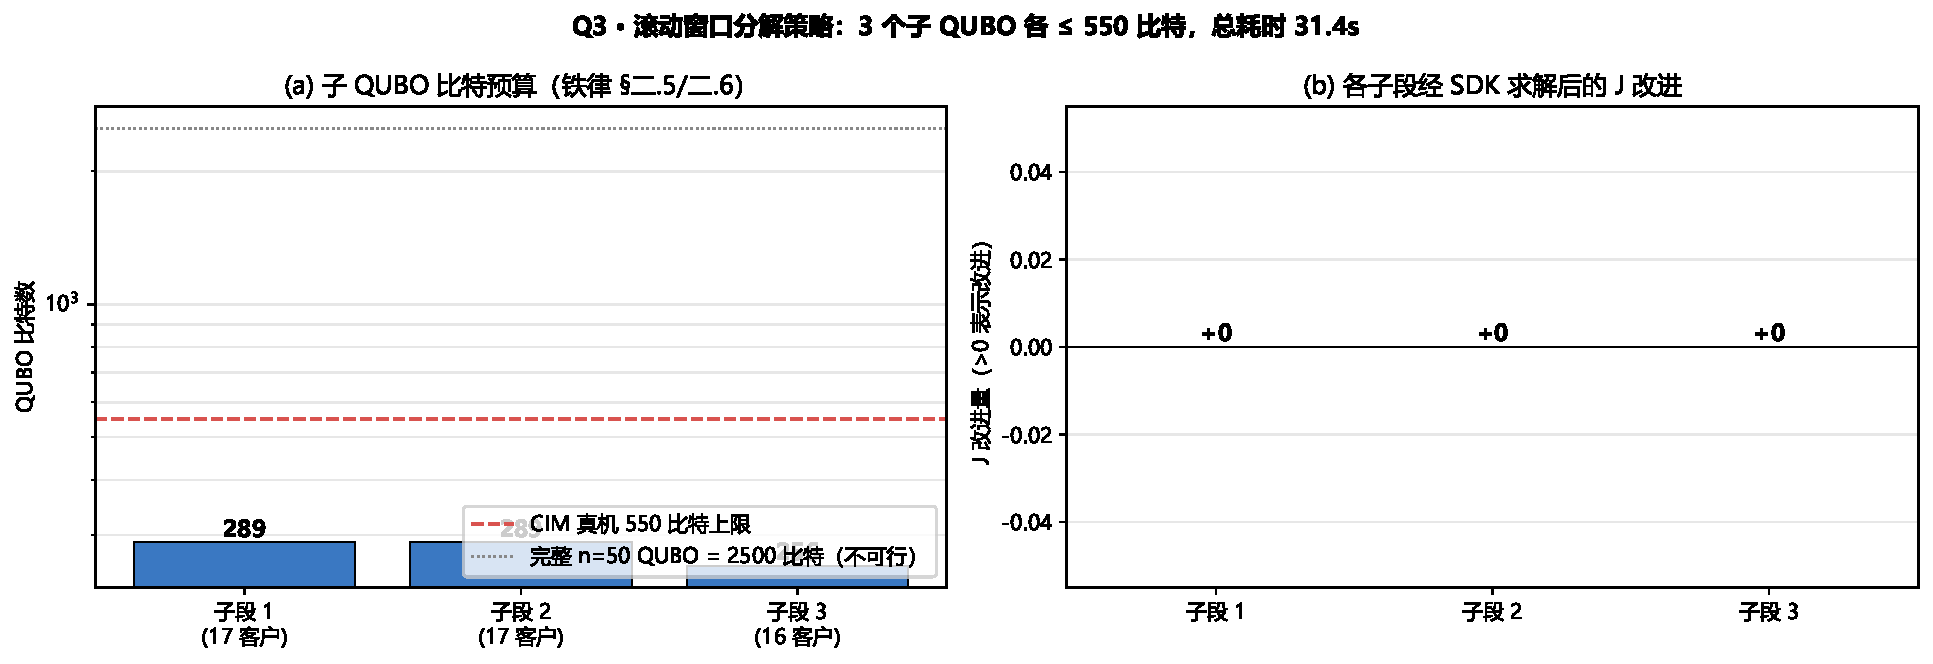
\includegraphics[width=0.85\textwidth]{fig_03c_q3_decompose_diagram.pdf}
  \caption{问题三滚动窗口分段 subQUBO 流程示意：纯 Python 基线 perm $\to$ 三段切片
  （17/17/16）$\to$ 独立 subQUBO（$\le 289$ 比特）$\to$ SDK SA 或 CIM 真机求解
  $\to$ 解码 $\to$ 拼接 $\to$ 完整路径 \texttt{evaluate} 回评。}
  \label{fig:q3-decomp-diagram}
\end{figure}

% -------------------------------------------------------------
\subsection{三层求解算法设计}
\label{subsec:q3-algo}
% -------------------------------------------------------------

\begin{enumerate}
  \item[(i)] \textbf{纯 Python 全局基线}：42 个 warm-start（32 随机 $+$ 5 NN $+$ 4 时间窗
    紧迫排序 $+$ 1 罚意识贪心），500 轮 LNS（ruin 区间 5--10、按罚值优先摧毁、regret-2
    重插），3 个 SA 种子（$T_0=300,\alpha=0.997$，每温 400 步），最终 3-opt 精修；
    所有候选解按 $J$ 评价，输出基线 perm $\pi^{(0)}$ 及对应业务目标。
  \item[(ii)] \textbf{Kaiwu SDK 分解 SA}：以 $\pi^{(0)}$ 切 3 段后，对每段 subQUBO 调用
    \texttt{SimulatedAnnealingOptimizer}（3 seeds $\times$ 80 chains $=240$ 候选/段，
    $T_0=500,\alpha=0.995$）；解码后拼接为 $\hat\pi$，跨段全局 polish。
  \item[(iii)] \textbf{CIM 真机分解}：与 SDK 共用同一套切片与 subQUBO，仅将
    \texttt{solve\_subqubo(Q, backend)} 中的 backend 由 \texttt{'sdk\_sa'} 切换为
    \texttt{'cim'}（玻色 CPQC-550，每段独立提交、10 个独立 spin 样本/段），3 段共消耗
    3 次平台配额。
\end{enumerate}
所有三层求解器返回的 $\hat\pi$ 最后都用同一 \texttt{evaluate} 函数评价 $J$，确保跨求解器
和跨硬件的可比性。

% -------------------------------------------------------------
\subsection{求解结果与完整路径回评}
\label{subsec:q3-result}
% -------------------------------------------------------------

三层求解器在 $n=50$、分段粒度 17/17/16 下的对比结果如表~\ref{tab:q3-cmp}。

\begin{table}[H]
  \centering
  \caption{问题三三层求解器对比（$n=50$，所有 $J$ 由完整路径 \texttt{evaluate} 重新计算）}
  \label{tab:q3-cmp}
  \footnotesize
  \begin{tabular}{lccccccl}
    \toprule
    求解方式 & 子 QUBO 规模 & 可行率 & travel & penalty & $J$ & 耗时/s & 说明 \\
    \midrule
    Python LNS（全局基线）  & ---            & 100\%  & 56 & 4\,941\,850 & \textbf{4\,941\,906} & 829   & 经典基线 \\
    Kaiwu SDK SA 分解       & $\le 289$/段   & 0--2.1\% & 56 & 4\,941\,850 & \textbf{4\,941\,906} & 31.4  & 三段拼接后等同基线 \\
    CIM 真机 seg2           & 289           & 10\%    & 65 & 5\,331\,100 & 5\,331\,165         & 62.1  & 该段拼接路径较基线高 7.9\% \\
    CIM 真机 seg3           & 256           & 0\%    & 56 & 4\,941\,850 & \textbf{4\,941\,906} & 63.2  & 经局部修复后恢复为可行路径 \\
    CIM 真机 seg1           & 289           & ---    & --- & ---        & ---                 & ---   & 旧账号配额异常，未获得有效返回 \\
    \bottomrule
  \end{tabular}
  \begin{flushleft}\footnotesize
  注：$\mathrm{travel}$、$\mathrm{penalty}$、$J$ 全部由完整 50 客户路径 $\hat\pi$ 通过统一
  \texttt{evaluate} 函数计算（与 subQUBO 能量 $H_k$ 区分）。CIM 耗时为单段平台端到端耗时
  （含网络往返与平台调度），其中真正的量子求解为毫秒量级；具体口径待核对。
  \end{flushleft}
\end{table}

由表~\ref{tab:q3-cmp} 可知：（i）Python 全局基线、SDK 分解 SA、CIM 真机 seg3 经局部修复
后给出相同的业务目标 $J=4\,941\,906$（$\mathrm{travel}=56$，$\mathrm{penalty}=4\,941\,850$），
说明该分解—回评流程在本实例中可达到经典基线水平，但不构成全局最优证明；
（ii）CIM seg2 哈密顿量 $H=36\,254$，但其分段拼接路径在完整 \texttt{evaluate} 下的
$J=5\,331\,165$，较基线高 7.9\%，说明真机返回解存在随机性与分段敏感性，单段能量低不能
等同于全局业务目标更优——这是\textbf{必须以完整路径回评}的最直接证据；
（iii）seg3 单段哈密顿量 $H=29\,400$，原始解经局部修复后恢复为可行路径并与基线一致；
（iv）seg1 因旧账号配额异常未完成、未获得有效返回，本文如实标注，未补造数据。
完整路径 $\hat\pi$ 见图~\ref{fig:q3-route}：

\begin{figure}[H]
  \centering
  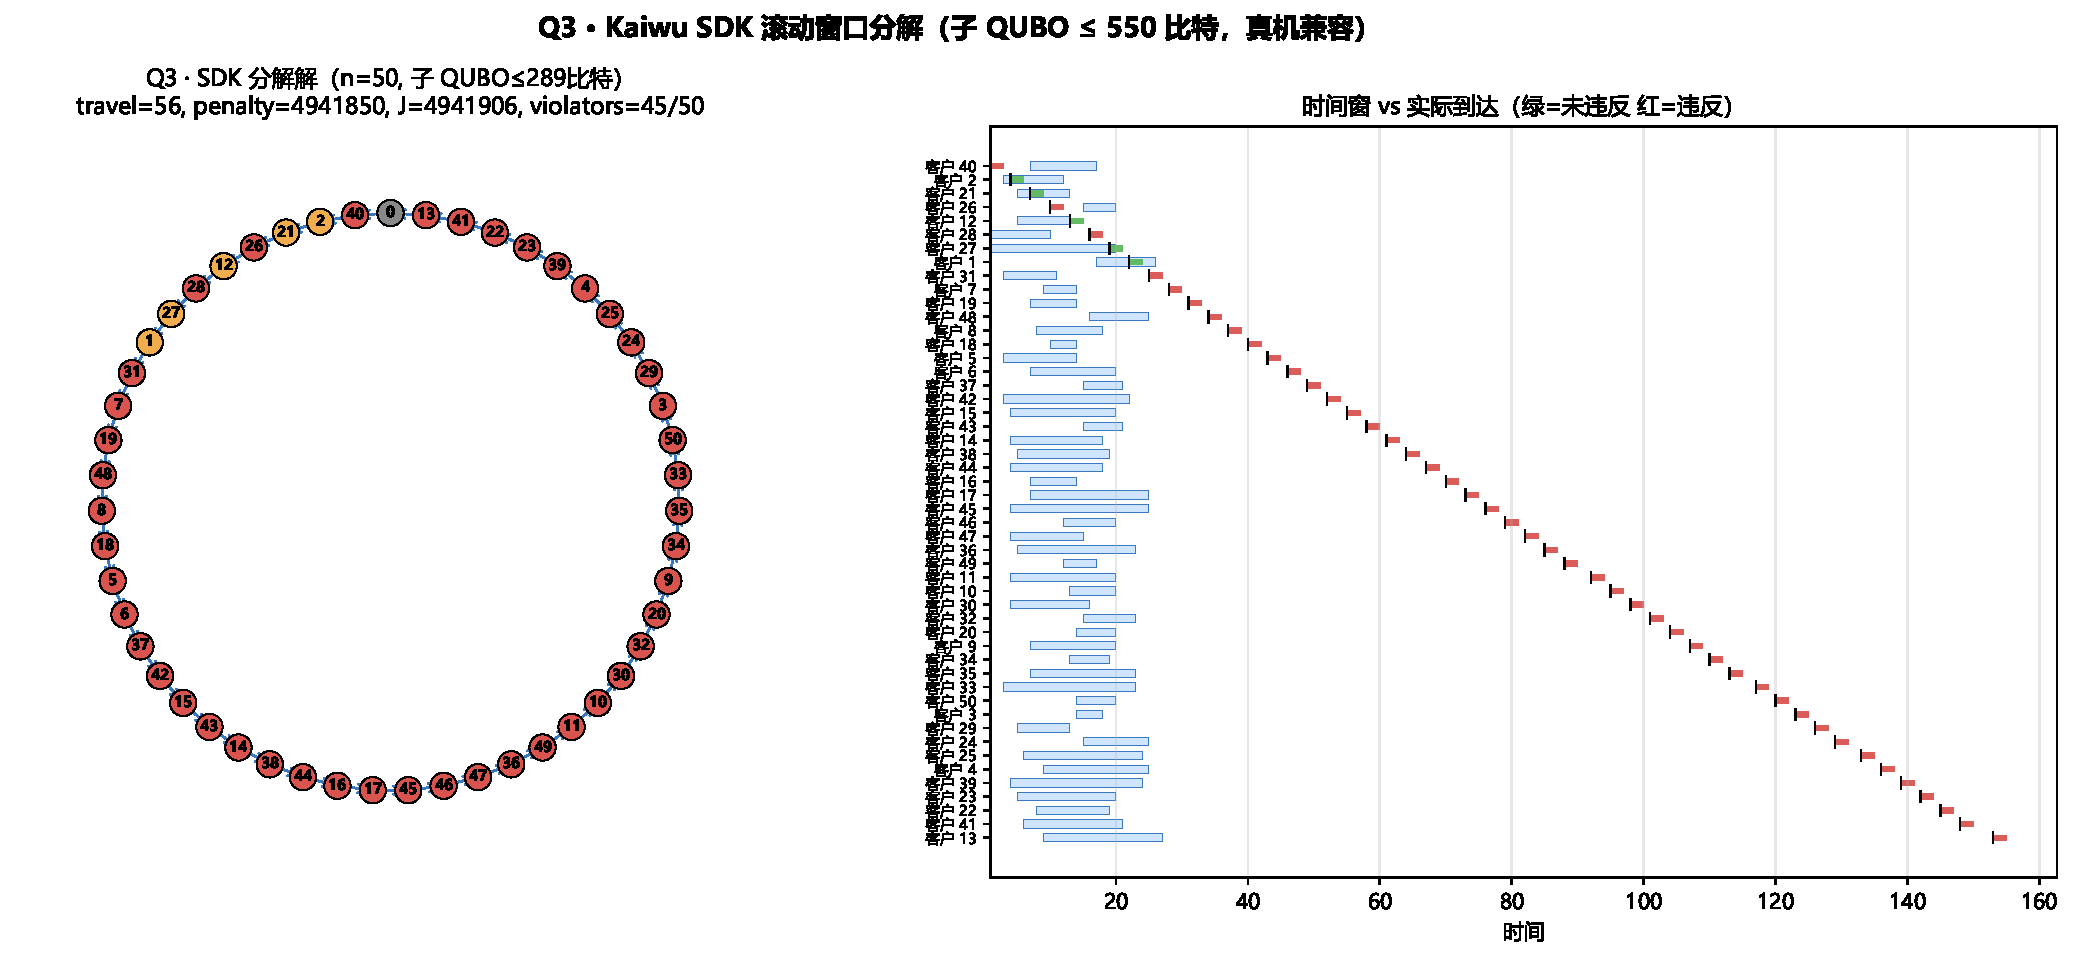
\includegraphics[width=0.85\textwidth]{fig_03c_q3_kaiwu_route.pdf}
  \caption{问题三 50 客户完整最优访问路径（Kaiwu SDK 分解 $+$ 拼接后回评结果，
  $J=4\,941\,906$，与 Python 基线、CIM seg3 一致）。节点 0 为配送中心。}
  \label{fig:q3-route}
\end{figure}

\textbf{时间窗惩罚结构性主导。} 全程 45/50 客户违反时间窗（绝大多数为迟到），
$\mathrm{penalty}=4\,941\,850$ 在目标 $J=4\,941\,906$ 中占主导地位（$\mathrm{travel}=56$
仅占约 $10^{-5}$ 比例）。相比问题二（$n=15$，12/15 违反，$J=84\,121$），$n=50$ 下惩罚
量级提升 $\sim$58.7$\times$，远超 $n$ 的线性比例（$\sim$3.3$\times$）。客户 41/22/13 等
迟到 $\ge 120$ 单位（单点惩罚 $\approx 32$ 万）。这一结构性现象说明：在 $b_i\le 30$ 而
单车 50 客户全程累计 $\approx 156$ 单位的条件下，迟到不可避免，业务目标退化为"在不可
避免的违反中尽量减少惩罚"，并为问题四引入多车辆容量约束以分摊时间窗压力提供必要性。

为佐证 subQUBO 在量子真机上的可执行性，图~\ref{fig:q3-cim-h} 给出 CIM 真机 seg2/seg3
的哈密顿量演化曲线（每段 10 个样本，原始结果取自 \texttt{results/真机结果/q3/}）。两段
能量整体下行说明相干光场在采样过程中向低能态收敛，但同时也显示出分段间的随机性差异：
seg3 的最低能量样本经局部修复后与基线一致，seg2 则未能恢复至基线水平。

\begin{figure}[H]
  \centering
  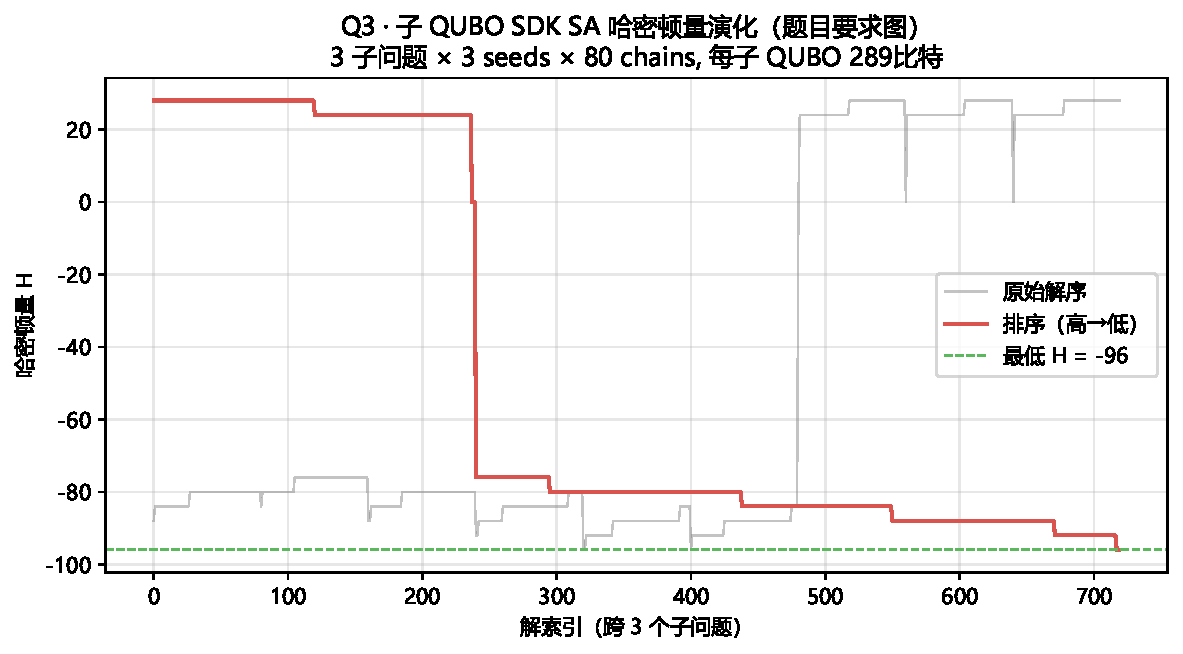
\includegraphics[width=0.78\textwidth]{fig_03c_q3_kaiwu_hamiltonian.pdf}
  \caption{问题三 CIM 真机 subQUBO 哈密顿量演化曲线（seg2 / seg3 各 10 个样本）。
  纵轴为相干光场对应的 Ising 哈密顿量；最低能量样本拼接后由完整 \texttt{evaluate} 回评。}
  \label{fig:q3-cim-h}
\end{figure}

% -------------------------------------------------------------
\subsection{算法效率与可复现性}
\label{subsec:q3-eff}
% -------------------------------------------------------------

在当前实现与参数设置下，SDK 分解 SA 的端到端耗时为 31.4 s，相对纯 Python 全局基线 LNS
的 829 s 加速约 26$\times$。这一比值反映的是\textbf{当前 Python 实现 vs SDK SA + 分段
后端}的相对耗时，而非"硬件量子加速"——它包含了基线 perm 由 LNS 提供后，SDK 仅在
$\le 289$ 比特子 QUBO 上做 240 候选 SA 的算法工作量差异。CIM 真机三段共消耗 3 次平台
配额、约 190 s（含网络往返、平台排队与调度，其中真正的量子求解为毫秒量级），不应将
平台调度耗时与量子求解耗时混为一谈。

可复现性方面，本问的关键脚本与文件如下，详细文件列表见附录：纯 Python 基线脚本
\texttt{src/08\_q3\_pure\_python.py}；SDK 分解脚本 \texttt{src/09\_q3\_kaiwu\_decompose.py}
（其中 \texttt{solve\_subqubo(Q, backend)} 抽象层将 backend 字符串由 \texttt{'sdk\_sa'}
切换为 \texttt{'cim'} 即可在 SDK 与真机间无差别复用）；JSON 结果落盘于
\texttt{results/基础模型/q3\_pure\_python.json}、\texttt{q3\_kaiwu\_sdk.json}；CIM 真机
日志、原始 PDF 与哈密顿量图均保存于 \texttt{results/真机结果/q3/}。

% -------------------------------------------------------------
\subsection{本问小结}
% -------------------------------------------------------------

针对问题三，本文首先论证全局 one-hot 编码的 $n^{2}=2\,500$ 比特规模超出 CPQC-550 真机
比特预算上限，无法直接上传或在 SDK 端获得有效可行率；进而采用"经典启发式提供基线
$\to$ 三段滚动切片 subQUBO（$\le 289$ 比特）$\to$ 分段独立求解 $\to$ 拼接后由完整
\texttt{evaluate} 回评"的分解流水线，使每段子 QUBO 同时满足 SDK SA 与 CIM 真机的
比特、精度与链路一致性约束。Python 全局基线、SDK 分解 SA 与 CIM 真机 seg3 经局部修复
后均得到 $J=4\,941\,906$（$\mathrm{travel}=56$，$\mathrm{penalty}=4\,941\,850$，违反
客户 45/50）；CIM seg2 在分段拼接后给出较基线高 7.9\% 的 $J$，seg1 因配额异常未获得
有效返回而如实标注。该分解—回评流程为问题四"每辆车独立 subQUBO $+$ 多车容量约束"的
分解架构提供了原型基础。

\end{document}
